\chapter{Introduction}
  % What is Louisiana, as a whole, in the public imagination
  % Why do we care about Louisiana
  % Objective: Examine how ethnicity and race are or are not expressed through subject pronouns in French and Creole as spoken in Louisiana
  \section{Fractal recursivity}
    % Definition
      % One of three semiotic practices used to "locate, interpret, and rationalize sociolinguistic complexity, identifying linguistic varieties with 'typical' persons and activities" (Irvine & Gal:36-37)
      % Specifically: a semiotic practice of distinction in which people project a salient opposition from one level to another, such as urban vs surburban into a smaller local context such as a school (Irvine & Gal 2000:38)
      % As a case of fractal recursivity, Irvine & Gal (2000) describe colonial Europeans imagining the sociolinguistic situation in Africa as being analogous to Europe's when mapping out the languages of the continent (49-55).
    % Previous work
  \section{Race and ethnicity}
    % Are these different concepts to begin with, and are they different from each other?
    \subsection{Race and ethnicity in the United States}
      % According to census records, the US has gone from 1 in 8 people being non-White to 1 in 4 (or 1 in 3 if Latinxs are treated as non-White) (Fischer & Hout 2006:25-26)
        % Ethnic and racial diversity, measured with Shannon entropy using census records, has increased between 1990 and 2010 (0.4576 > 0.6015) (Wright et al. 2014:175)
        % The pattern holds through the 2020 census except for non-Whites increasing to 42% of the population when treating Latinxs as non-White (Census 2020)
        % "[R]oughly half" of White Americans thought they were a minority already by 2000 (Alba et al. 2005, as cited in J. A. Smith et al. 2014:437)
      % Latinx is currently the largest non-White group (19.5%) followed by Blacks (13.7%) (Census 2020)
        % Growth in the Latinx population in 2011 was driven more by births than by immigration (Pew Hispanic Center 2011, as cited in Wright et al. 2014:181)
      % According to censuses, between 1990 and 2010, White-dominant neighborhoods decreased from 66.0% to 42.5% (i.e., diversity increased) (Wright et al. 2014:176)
      % Most immigrants settled in highly populous metropolitan areas according to the 2000 and 2010 censuses (75%) (Wright et al. 2014:175)
      % Attitudes have moved towards greater tolerance of racial and ethnic minorities from the 1970s to the 2010s (Bobo et al. 2012; Firebaugh & Davis 1988, both as cited in J. A. Smith et al. 2014:437)
      % Racial income inequality decreased earlier in the 20th century but stalled by 2000 (Leicht 2008, as cited in J. A. Smith et al. 2014:436)
    \subsection{Race in Louisiana}
      % The increase in the Latinx-dominant neighborhoods in the US has mostly occurred in the western states (i.e., not Louisiana), according to census records between 1990 and 2010 (Wright et al. 2014:179)
    \subsection{Cajun identity}
      % Study participants in St Landry identifying as Cajun (N = 9) all also identified as White (Klingler 2003 "Language":82)
    \subsection{Creole identity}
      % Study participants in St Landry identifying as Creole (N = 19) all also identified as Black (Klingler 2003 "Language":82)
    \subsection{Language ideologies accounting for race or ethnicity}
      % Study participants in St Landry claimed to speak French if they identified as Cajun and Creole if they identified as Creole, regardless of whether their speech appeared structurally more like French or more like Creole (Klingler 2003 "Language"), but Louisiana isn't the only place where race and ethnicity influence language ideologies.
      % During the Quiet Revolution in Quebec, one might hurl an insult at people speaking French in public by demanding that they "speak White" (i.e., English) instead (Lamarre 2014:149)
    \subsection{Racially conditioned language variation}
    \subsection{Ethnically conditioned language variation}
  \section{French and Creole}
    % Glossonym
      % Creole speakers in Pointe Coupee (determined by the language structure) mostly call their language "créole" but sometimes also "français" or "cadien", though even when using the latter two glossonyms, speakers note that their language isn't like French from France or Cajun from Lafayette (Klingler 2003 "Turn":128)
    % Where is situated socially and geographically?
    \subsection{Status in Louisiana}
      % Where did French come from in the first place
        % Although Acadian French is at least implicitly considered the main origin of French in rural Louisiana, there are many sources for French (Klingler 2009)
        % Gudmestad & Carmichael (2022) had a number of study participants (Indians) who were native speakers in their 30s (in 2007-2008) in Terrebonne-Lafourche (6-7)
    \subsection{French vs Creole}
      % French and French-related varieties that exist
        % "Cajun French" (though he prefers "Louisiana Regional French" as it is not spoken purely by Cajuns), "Louisiana Creole", and "Colonial French" (which he and Picone (1998) prefer to call Plantation Society French since it developed in the 19th century) (Klingler 2003 "Language":77)
      % Speakers' approaches to naming their languages as one or the other
        % When asked plainly (without pushing for greater specificity), speakers of both varieties in St Landry will call their language "French" (Klingler 2003 "Language":78-79)
        % It's not unusual to place languages under a label based on cultural traits of the speakers rather than the structure of their ways of speaking
          % Linguists once described Cangin as a variety of Sereer because Wolofs in the area saw the cultural practices of both Cangin and Sereer speakers as being the same (Irvine & Gal 2000:57)
      % Structural blurring of boundaries between French and Creole
        % This is particularly prevalent in Lafayette, Breaux Bridge, and Vacherie (Klingler 2003 "Language":78), the former two being where much of my data comes from.
        % Klingler (2003 "Language") uses 1sg subject pronouns, past perfective constructions, and the verb 'to have' as diagnostics for structurally disentangling French and Creole (80)
    \subsection{Distinguishing features}
      % Geographic variation
        % Almost all of the variants marked as Creole (by Klingler, 1sg subject pronouns, perfective aspect representation, and the verb 'to have') used by speakers in St Landry Parish were produced by 4 speakers from Leonville, Prairie Ville, and Arnaudville (Klingler 2003 "Language":83).
          % Most variants were marked as French in general
          % Most Creole variants were also used by Blacks, though not exclusively (some White Cajuns used Creole-marked perfective aspect)
        % Almost all variants of 1sg pronouns, perfective aspect, and the verb 'to have' used by speakers in Pointe Coupee (3 Black, 2 White) were variants marked as Creole save for some tokens (~7%) of 'avoir' used only by Whites (Klingler 2003 "Language":81)
    \subsection{Subject pronoun system}
      % Terrebonne-Lafourche
        % For 1sg, null was the most common for Indian speakers of all levels, sometimes with moi (i.e., moi by itself was possible) (Gudmestad & Carmichael 2022:11)
      % Not Terrebonne-Lafourche
    \subsection{Racially and ethnically conditioned pronouns} % Add general social and structural constraints to pronoun predictors chapter
      % 1sg as [z] in Terrebonne-Lafourche may be indicative of Indian identity (Dajko 2009, as cited in Gudmestad & Carmichael 2022:5)




      
  % Everything above here has been put in the appropriate section ---------------------------------------





  % The idea of Louisiana in the public imagination is most often that of South Louisiana and the New Orleans metropolitan area, the former as shown in Figure \ref{fig:south_la} and the latter just east of the South Louisiana outline on the southern border of Lake Pontchartrain.
  % Indeed, the boundary between North and South Louisiana is traditionally a division in culinary practices, religion, and language \parencite[p.~309]{trepanier_french_1988}, where those cultural features that most distinguish Louisiana from the rest of the Deep South are those of South Louisiana.
  % % This has led to a situation where even South Louisiana locals will sometimes derisively refer to North Louisiana as ``South Arkansas'', a reference to the perceived indistinguishability of North Louisiana from the rest of the mostly Anglo, Protestant American South.
  % % Gold (1979) also describes North Louisiana as ``anglophone'' (265), and Johnson (1976) describes Northerners as historically being ``rabid anti-Catholic Protestants'' (27).
  % For sociolinguists, South Louisiana is of interest for two reasons: The two major local ethnic categories -- Creole and Cajun -- have over time been redefined to align with the Black and White American racial binary, respectively, and French is spoken there as a heritage language where it was the dominant language as recently as the mid 20th century.

  % \begin{figure}[tbhp]
  %   \centering
  %   \caption{Map of South Louisiana, also referred to as Acadiana}
  %   \label{fig:south_la}
  %   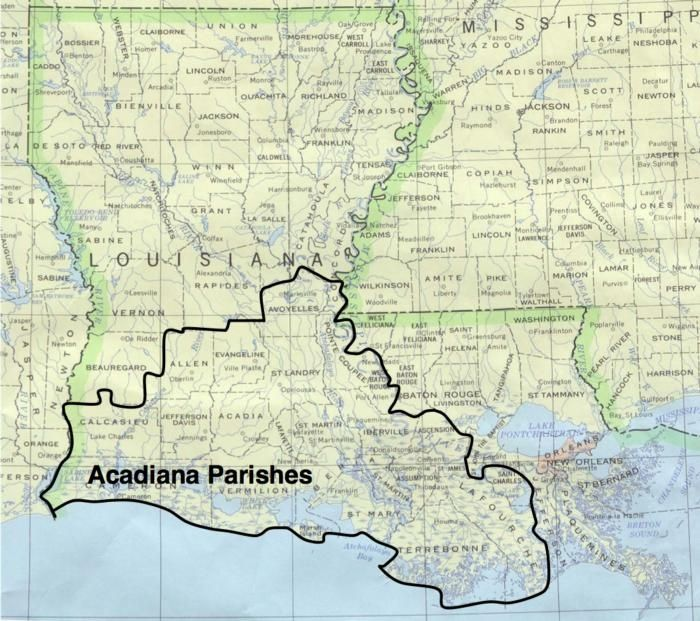
\includegraphics[scale=0.35]{acadiana.jpg}
  %   % Should identify Acadiana, New Orleans, but also Lafayette and Terrebonne-Lafourche
  % \end{figure}

  % This context provides an opportunity to better understand the salience and persistence of local ethnic categories both in the face of the imposition of broader racial categories and in a linguistically tenuous situation.
  % In particular, this study will focus on whether and to what extent the general social segregation of Black and White Americans in the United States \parencite{smith_social_2014} has been recapitulated between Creoles and Cajuns and found expression in the linguistic patterns of Creoles and Cajuns.
  % This subject will be approached by submitting data collected from around Lafayette Parish in South Louisiana to traditional variationist methodology, social network analysis, and textual analysis centered around subject pronouns as linguistic variables, as these have been found to vary along ethnic lines in other contexts \parencite{dajko_ethnic_2009, rottet_language_1995}, and ethnicity and race as the primary social variables.

  % \section{Ethnicity and race in South Louisiana}
  %   \label{sec:ethnicity_race}
  %   The complexity of ethnicity in South Louisiana is perhaps due to the variety of colonizing forces that have controlled it as well as immigration patterns.
  %   It was initially colonized by France, who turned over control to Spain in the 1760s, who then gave control of the region back to France very shortly before France sold it to the United States in the Louisiana Purchase of 1803 \parencite{fortier_french_1884, johnson_louisiana_1976, klingler_if_2003}.
  %   Additionally, Louisiana has been the landing point for influxes of people from Saint-Domingue\footnote{
  %     Present day Haiti.
  %   } after the slave revolts \parencite[Debien \& Le Gardeur, 1981, as cited in][]{klingler_if_2003}, Acadia\footnote{
  %     Roughly the present-day provinces of Nova Scotia and New Brunswick in Canada.
  %   } after the mass expulsion known as the \foreign{Grand dérangement} \parencite{fortier_french_1884, klingler_if_2003, neumann_creole_1985}, and even the Canary Islands \parencite{klingler_if_2003}.
  %   The result has been the formation of two general South Louisiana ethnic categories -- Cajun and Creole -- which have come to be redefined by the introduction of the Black-White racial binary of the United States \parencite{dajko_sociolinguistics_2012}.
  %   The overarching goal of this study is to better understand, through the lense of French subject pronoun variation, to what extent this racial binary has led to similar boundaries being drawn between Cajuns and Creoles, and so it is important to understand how Cajuns and Creoles have been defined.

  %   % \subsection{Cajuns}
  %   %   \label{sec:cajuns}
  %     The typical description of Cajuns is that of a poor, isolated, and stigmatized people.
  %     This negative evaluation, however, began shifting towards being more positive in the 1960s with the establishment of the Council for the Development of French in Louisiana (CODOFIL) \parencite[pp.~31-33]{brown_pronominal_1988}, which also brought with it the Americanization of the group.
  %     Criteria for membership once included speaking French, being rural, being Catholic, and especially having Acadian ancestry \parencite{johnson_louisiana_1976, neumann_creole_1985, smith_influence_1939}.
  %     The assimilation of South Louisiana into the broader American culture, however, has brought with it the American Black-White racial binary resulting in a shift towards membership being strongly based on being White.
  %     For instance, research participants who self-identify as either Creole or Black have been reported as often defining Cajuns as White and Creoles as Black \parencite[p.~34]{giancarlo_dont_2019}, which has been the case even for participants who have acknowledged that Cajuns may be darker skinned Whites and Creoles may be lighter skinned Blacks \parencite[Stanford, 2016, as cited in][p.~32]{giancarlo_dont_2019}.

  %     % Scholars in the early 20th century tended to claim that Cajuns were generally immobile \parencite[e.g.,][]{smith_influence_1939}.
  %     %, which may explain why they were once called the nation's ``largest unassimilated minority'' \parencite[Gilmore, 1933, as cited in][p.~99]{rottet_language_1995}: without opportunities to interact with outsiders, there was little chance that they would assimilate to those outsiders.
  %     % Although Cajuns will sometimes claim the uniqueness of their culture that stems from this lack of assimilation as a badge of honor, it has also resulted in them once being thought of as ``poor white trash'' \parencite[p.~110]{rottet_language_1995}.
  %     %  as well as the broader American population and French people becoming more interested in the region
  %     % Of course, with this increased contact with outsiders has also come increased Americanization and a loss of the uniqueness of culture that Cajuns prize, which includes the French language.
  %     % Specifically, it has been claimed that assimilation into the broader American culture has been thrust forward first by compulsory education, then by the advent of mass communication, followed by involvement in World War II, and finally by the Louisiana oil boom that drew many new people to the state \parencite[Conrad, 1978, as cited in][p.~28]{brown_pronominal_1988}.

  %     % Along with the changes in Cajun culture and social evaluations of Cajuns have come changes in the criteria for membership into this ethnic group.
  %     % In the early 20th century, several conditions needed to be met in order to be considered Cajun.
  %     % Chief among them was the abililty to speak French \parencite[p.~198]{smith_influence_1939}, though others have also noted the importance of being rural and Catholic \parencite[Del Sesto \& Gibson, 1975, as cited in][p.~15]{neumann_creole_1985}.
  %     % Indeed, this criteria is not far off from those used by \textcite{trepanier_french_1988} to distinguish between North and South Louisiana, as mentioned in the introduction.
  %     %
  %     % Another condition that allows one to claim Cajun as their ethnicity is ancestry, specifically ancestry that can be traced back to Acadia from before the \foreign{Grand dérangement} \parencite[p.~19]{johnson_louisiana_1976}.
  %     % Indeed, the term \lexi{Cajun} itself originated in mispronunciations of the term \lexi{Acadian} \parencite[p.~198]{smith_influence_1939}.
  %     % Although the link is not obvious in English, \lexi{Acadian} in French is \lexi{acadien} [akadjɛ̃], which Acadians as well as French-speaking Cajuns today pronounce as [akadʒɛ̃], making it quite close to the English pronunciation of \lexi{Cajun} as [keɪdʒən].
  %     % This close connection with Acadia is so strong that even recent scholars have implied that ancestry is what should ideally define someone as Cajun as \textcite{giancarlo_dont_2019} did when arguing that the parishes\footnote{
  %     %   A parish is the Louisiana equivalent of a county in other states.
  %     % } of St Landry and Lafayette are not actually dominated by Cajuns as Acadian surnames are not common there.
  %     % \textcite{giancarlo_dont_2019}, citing Brasseaux (1992) and Stanford (2016), did acknowledge that surnames are not reliable for identifying ancestry as Acadians/Cajuns have intermarried since their arrival in Louisiana and Cajuns today trace their ancestry matrilineally (p.~33).
  %     % Furthermore, although the importance of ancestry continues to be given as a defining feature of Cajun group membership, it ceased being a hard requirement since at least the 1980s \parencite[pp.~18-20]{brown_pronominal_1988}.
  %     % It appears, then, that Acadian ancestry is perhaps a sufficient condition for being Cajun on its own, but it is not a necessary conditon today.
  %     %
  %     % Another condition for Cajun membership that is entangled with ancestry and has come to all but subsume the other conditions is race.
  %     % At one time, Louisiana society's racial classification of Cajuns was somewhat ambiguous as they were considered to be better than Black but not quite White \parencite[Tentchoff, 1980; Walton, 2003, as cited in][p.~32]{giancarlo_dont_2019}.
  %     % For instance, Spitzer (1977) and Esman (1985) both identified Blacks as participating in Cajun\footnote{
  %     %   There is of course much debate over which cultural traditions in Louisiana are Cajun and which are Creole \parencite{giancarlo_dont_2019} as well as who is Black and who is not \parencite{susberry_racial_2004}, but Spitzer and Esman's reports remain enlightening either way.
  %     % } culture yet not referring to themselves as Cajun \parencite[as cited in][p.~43]{brown_pronominal_1988}.
  %     % As will be shown in the next section, just as the term \lexi{Cajun} has become more or less synonymous with White South Louisianian, so too has \lexi{Creole} become synonymous with Black South Louisianian.

  %     % Giancarlo (2019) makes the point that this is actually harmful in the sense that there is ethnic diversity in this population of non-Creoles that has all been collapsed into "Cajun" (33).
  %       % That's not to say there are not acknowledged distinctions, though, as locals sometimes distinguish between Prairie Cajuns and Bayou Cajuns (R. A. Brown 1988:74-75).

  %   % \subsection{Creoles}
  %     The definition of Creoles has changed even more dramatically over time than the definition of Cajuns.
  %     In the early colonial history of Louisiana, the term Creole was applied to White people of French and Spanish descent (\citeauthor{fortier_french_1884}, \citeyear[p.~98]{fortier_french_1884}; \citeauthor[Kein, 2000, as cited in][]{susberry_racial_2004} \citeyear[pp.~7-8]{susberry_racial_2004}), matching how some still define Creoles today.
  %     Free, mixed-race people were not at that time called Creoles but were rather derisively called mulattos, quadroons, and octoroons.
  %     The negative stigma associated with these terms, however, led Free People of Color to eventually co-opt the term Creole for themselves \parencite[Martin, 2000, as cited in][pp.~7-8]{susberry_racial_2004}, creating a three tier racial system that consisted of Whites at the top, Creoles in the middle, and Blacks (i.e., those who were enslaved) at the bottom.
  %     By the 20th century, though, there were strong societal forces in Louisiana pushing to have mixed-race Creoles identified simply as Black, which some resented \parencite[pp.~12-13]{susberry_racial_2004}.
  %     The result is a situation today in which Creoles may racially define themselves any number of ways, such as White, Black, Creole, fluid, etc. \parencite{susberry_racial_2004}, though society likely treats them all as simply Black.
  %     Like with Cajuns, where part of the definition of a Creole also included being francophone or creolophone \parencite[p.~11]{neumann_creole_1985}, the racial criteria for membership has effectively subsumed all others.

  %     % Members of the ethnic group today might define Creoles as being descendants of the original French and Spanish colonists in Louisiana, especially if Africans or Native Americans are found in that line of descent, or simply being multiracial people from South Louisiana \parencite[p.~56]{susberry_racial_2004}.
  %     % A common thread in all definitions, though, is the idea that Creoles are necessarily ``not Cajun'' \parencite[pp.~26/42]{giancarlo_dont_2019}, suggesting that they are defined as the Other.
  %     % Today, many of Louisiana's cultural exports and landmarks have been branded as Cajun to the detriment of the role of Creoles and sometimes even their authorship \parencite{giancarlo_dont_2019}.
  %     % Despite this branding that erases Creoles from the landscape, local interest in Creole identity has persisted.
  %     % This is perhaps a reaction to said branding, but other factors involved in this continued interest have also been noted, such as the census finally allowing Creoles to not have to identify as Black, the push for French language education, and the popularity of geneological research \parencite[p.~14]{susberry_racial_2004}.

  %     % This later came to include those coming to Louisiana after the slave revolts in Saint-Domingue at the turn of the 19th century (\citeauthor{neumann_creole_1985}, \citeyear[p.~11]{neumann_creole_1985}; \citeauthor{rottet_language_1995}, \citeyear[p.~6]{rottet_language_1995}).
  %     % In fact, by that time, the term Creole not only applied to people originating in Louisiana but even foods and other objects \parencite[p.~21]{johnson_louisiana_1976}.
  %     % As \textcite{neumann_creole_1985} noted, whereas Creoles were understood to be Black or mixed-race francophones early in the century, they came to be understood as Black creolophones by the 1980s (p.~11), bringing the more stigmatized language variety of Louisiana Creole into the fold (pp.~23-25), as well.\footnote{
  %     %   Neumann reported that English was the most prestigious variety in Louisiana at the time, followed by the local variety of French, and finally the closely related Louisiana Creole.
  %     % }
  %     % Some Creoles resented being collapsed in with Blacks and so either attempted to pass as White if they were light skinned enough or otherwise became activists pushing for Creoles to continue to be seen as a distinct group \parencite[pp.~12-13]{susberry_racial_2004}.
  %     % In any case, what is clear from these definitions is that, despite \lexi{Creole} perhaps being best thought of as an ethnic label, race has always been a central aspect of historical definitions: Creoles began as Whites from Europe who were born in Louisiana before later being mixed-race free people.
  %     %
  %     % While Creoles in the 21st century may still be seen as mixed-race by Louisianians, in the context of American society where everything is either White or Black or at least White or Other, Creoles are not necessarily precluded from being treated as \foreign{de facto} Black as opposed to being in a third racial category.
  %     % This binarity is so pervasive that even activists and researchers who are purposefully holding onto a mixed- or third-race identity for Creoles will sometimes fall back into the binary.
  %     % For instance, \textcite{giancarlo_dont_2019} cited such activists and researchers as arguing that much of South Louisiana's local culinary traditions are in fact Creole and not Cajun because slaves would have been doing the cooking when these traditions began (pp.~39-40).
  %     % However, this presumes that slaves were Creoles, though at the time of slavery, they were not considered Creoles but were instead considered Black, treated as a notch below Creoles of Color and well below the White Creoles during the early colonial days.

  %     % Susberry (2004) examined how self-identified Creoles (of color) characterized themselves racially using Rockquemore's (1999) biracial model.
  %       % The possible racial identities were Black, Protean (i.e., shifting), and Border (i.e., biracial) (Susberry 2004:33).
  %     % As already noted, many of Giancarlo's Creole informants (of color) characterized Cajuns as White and Creoles as Black (34).

  % \section{Louisiana French}
  %   Some Cajuns and Creoles do still speak French today, despite this no longer being a necessary criteria for membership, though it is likely a sufficient criteria for membership when met.
  %   The French variety that would gain one access to membership in one of these groups is specifically Louisiana French, which is sometimes also referred to as Cajun French\footnote{
  %     It is somewhat of a \foreign{faux pas} to use this term today as it presumes that all speakers are Cajuns and all non-Cajuns are non-speakers, though even local francophones will still sometimes use the term.
  %   }.
  %   Traditionally, there have in fact been three French-based language varieties delineated in Louisiana: Colonial or Plantation French, Louisiana French, and Louisiana Creole.
  %   Colonial French is thought to be all but extinct but was spoken primarily by recent French immigrants after the Louisiana Purchase.
  %   While there are still francophone immigrants coming to Louisiana even today, they have not coalesced around a variety that might still be called Colonial French but have instead continued to speak a wide range of French varieties.
  %   Louisiana French is the French variety that was the dominant language of rural South Louisiana up until the mid 20th century.
  %   Finally, Louisiana Creole is a French-based creole that has similarities with other Atlantic French-based creoles such as Haitian Creole but is not likely to be related to them \parencite[pp.~280-281]{dajko_sociolinguistics_2012}.

  %   The linguistic focus of this study will be on ethnic variation in subject pronouns in Louisiana French, the variety being broadly defined, meaning Louisiana Creole will not be excluded as these two varieties are quite close structurally, particularly in the parishes that are adjacent to Lafayette Parish where participants will be sought out.
  %   Indeed, in cases of code-switching between Louisiana French and Louisiana Creole, it can be extremely difficult to distinguish where one variety ends and another begins \parencite{klingler_probleme_2005} as there are very few lexical differences (\citeauthor{neumann_creole_1985}, \citeyear[p.~52]{neumann_creole_1985}; \citeauthor[Rottet, 2000, as cited in][]{klingler_probleme_2005}, \citeyear[p.~352]{klingler_probleme_2005}).
  %   It has also been noted that Louisiana French displays syntactic features that are closer to Louisiana Creole than other varieties of French in parishes where the two are in contact \parencite{baronian_influence_2005}.
  %   Furthermore, speakers and sometimes even researchers have defined these two varieties more by who the speaker is than by their linguistic structures in the sense that Creoles are said to speak Louisiana Creole even when their speech patterns resemble French and Cajuns are said to speak Louisiana French even when their speech patterns resemble Creole (\citeauthor{brown_pronominal_1988}, \citeyear[p.~5]{brown_pronominal_1988}; \citeauthor{klingler_language_2003}, \citeyear{klingler_language_2003}).
  %   Given these facts as well as claims that the two varieties are mutually intelligible \parencite[p.~29]{neumann_creole_1985}, excluding Louisiana Creole would be difficult at best and questionable at worst, and so ``Louisiana French'' here may include speech that appears Creole-like.

  %   Louisiana French differs from varieties of French spoken outside of Louisiana in several ways, but there is also variation within Louisiana itself.
  %   Some of the more salient features that set Louisiana French apart from varieties such as Quebec French or Hexagonal French\footnote{
  %     French as spoken in France.
  %   }, though some of these features can appear in other varieties, include an explicit progressive construction using the preposition \lexi{après} as in Sentence \ref{sent:progressive} \parencite{papen_structural_1997}, /ʒ/ produced as [h] \parencite{carmichael_language_2019, papen_structural_1997}, the flap [ɾ] where most varieties have [ʀ] or [ʁ] \parencite{blainey_first_2013}, and importantly for the present study, a unique subject pronoun system that includes items such as \lexi{ça} being used for animate 3rd person plural referents whereas this pronoun is generally reserved for inanimate singular referents in other varieties \parencite{dajko_ethnic_2009, rottet_language_1995}.
  %   The subject pronoun system is one that has been found to be variable within Louisiana French itself, as will be discussed in detail below.
  %   \begin{enumerate}
  %     \item \label{sent:progressive}
  %       \begin{tabular}[t]{l l l l}
  %         il & (est) & après & manger \\
  %         he & is    & after & to eat \\
  %         \multicolumn{4}{l}{\gloss{He is eating.}}
  %       \end{tabular}
  %   \end{enumerate}

  %   % R. A. Brown (1988) defines the 3 French-based languages of Louisiana -- Colonial, Cajun, and Creole -- as being spoken by European Creoles, Acadian descendants, and descendants of slaves, respectively (34-35), suggesting that even researchers have defined these varieties by who their speakers are rather than by linguistic structure.
  %   % Baronian (2005) claims that both Cajuns and Creoles in Vermilion Parish speak a variety of French, whereas in St Martin Parish, Cajuns speak French and Creoles speak Creole (134-135).
  %     % The differences between French and Creole are very slight and include mo vs je and gen vs avoir.

  %   % Other "languages" present
  %     % Two years of elective Standard French courses were available even in the 1930s (Smith & Philips 1939:199).
  %       % Well, they don't say "Standard", but that can probably be assumed.
  %     % Code-switching is not only present between French and English (B. Brown 1986) but even between French, English, and Creole (Klingler 2005), not to mention English lexical borrowings starting at least as early as the first decades of the 20th century (Smith & Philips 1939).
  %       % As for French-Creole bilinguals, Neumann (1985) claims that they were few and mostly White (29).

  %   % Status
  %     % Finally, as for the status of Louisiana French, the language was not long ago dominant in rural South Louisiana but is today likely considered a heritage language.
  %     % It is oft repeated that estimates of French speakers in the state are hard to obtain -- for instance, the US census once gave only the option of ``French'' but not specifically local varieties of French when choosing the language spoken at home, and speakers sometimes equated ``French'' to International varieties and not their own variety \parencite[p.~98]{brown_social_1993} -- and so the numbers given over the years have varied widely.
  %     % CODOFIL (1969) suggested there were 1,484,440 speakers in the 1960s, whereas Smith-Thibodeaux (1977) estimated 300,000-500,000 and Neumann (1985) 500,000-1,000,000 \parencite[as cited in][p.~113]{rottet_language_1995}.
  %     % There is consensus, though, that the number of French speakers in Louisiana is generally dwindling.
  %     % For example, though \textcite{rottet_language_1995} had no real difficulty finding francophone Houma Indians under the age of 30 in his study of Southeast Louisiana, he had much more difficulty finding Cajuns in this age group who spoke French (p.~71).
  %     % Americanization, as discussed in Section \ref{sec:ethnicity_race}, and general economic pressures from the oil boom that brought in many Texans and anglophone North Louisianians have been cited as reasons for the decline in French (\citeauthor{neumann_creole_1985}, \citeyear[p.~49]{neumann_creole_1985}; \citeauthor[Larouche, 1981, as cited in][]{rottet_language_1995}, \citeyear[p.~105]{rottet_language_1995}), but whatever the cause, it is readily apparent that there are fewer speakers each day.

  %   % New Orleans is somewhat excluded from definitions of South Louisiana because it differs in several respects culturally, and one of those is the lack of locally grown French varieties.
  %     % Johnson (1976) argued that there were maybe 5,000 "indigenous speakers" of French in New Orleans at the time (23).
  %   % There has long been consensus, though, that the number of French speakers is generally dwindling
  %     % Neumann was actually talking about the decline of Louisiana Creole.
  %     % The large migration OUT of Louisiana to Texas during the earlier 1900s oil boom in the latter (Louder & Leblanc 1983, as cited in Rottet 1995:16) may have also helped galvanize the march towards English in Louisiana.

  %   \subsection{Ethnicity and subject pronouns}
  %     Subject pronouns in the French spoken in South Louisiana, summarized in Table \ref{tab:lf_sub_pro}, have previously been found to vary according to the ethnicity of the speaker \parencite{rottet_language_1995, dajko_ethnic_2009}, though the ethnic groups included in these studies have been Cajuns and Houma Indians, who have not been oppositionally racialized in the way Cajuns and Creoles have.
  %     The results from these previous studies demonstrate however that subject pronouns can work as indexicals on some level in Louisiana French.
  %     Furthermore, as working with Creoles also implicates Louisiana Creole and the subject pronouns often associated with that variety, as will be discussed below, subject pronouns would be a likely place to find expression of a Black-White segregation being applied to Cajuns and Creoles if such a segregation exists.

  %     % Phonetic stuff
  %       % The 1st person singular pronoun also involves phonetic variation in that three different consonants may be used in the pronunciation so that one might hear [ʒə], [hə], or [zə], all of which may also be metathesized.
  %       % There is additionally a phonological process which causes devoicing of the consonant when followed by a voiceless consonant in the verb \parencite{carmichael_language_2019}.
  %       % Some of the other pronouns that are also subject to their own notable phonetic variations are \lexi{vous} ([vu], [u], or [vo]), \lexi{elle} ([ɛl] or [al]), \lexi{nous} ([nu] or [no]), \lexi{vous-autres} ([vuzɔt], [uzɔt], or [zɔt]), and \lexi{eux} ([øs], [ø], [øz], or [zø]).
  %       % Finally, the final segments of practically all of these subject pronouns are dropped in certain linguistic contexts.
  %       % While it will be useful to keep in mind the existence of these phonetic variations, the present study will focus on morphosyntactic variation and so collapse these phonetic variants appropriately into individual lexical items during analysis.

  %     \begin{table}
  %       \centering
  %       \caption{The subject pronoun system of Louisiana French}
  %       \label{tab:lf_sub_pro}
  %       \begin{tabular}{l l l}
  %                   &                                          & \\
  %         Variable  & Description                              & Variants \\
  %         \hline
  %         (1sg)     & 1st person singular                      & \lexi{je}, \lexi{mo}, ø \\
  %         (2sg.T)   & 2nd person singular T form               & \lexi{tu}, \lexi{to} \\
  %         (2sg.V)   & 2nd person singular V form               & \lexi{vous}, \lexi{tu}, \lexi{to} \\
  %         (imp)     & Impersonal pronoun                       & \lexi{on}, \lexi{tu}, \lexi{vous}, \lexi{to} \\
  %         (3sg.AF)  & 3rd person singular animate feminine     & \lexi{elle}, \lexi{li} \\
  %         (3sg.AM)  & 3rd person singular animate masculine    & \lexi{il}, \lexi{li} \\
  %         (3sg.IF)  & 3rd person singular inanimate feminine   & \lexi{ça}, \lexi{elle}, \lexi{li} \\
  %         (3sg.IM)  & 3rd person singular inanimate masculline & \lexi{ça}, \lexi{il}, \lexi{li} \\
  %         (expl)    & Expletive pronoun                        & \lexi{il}, \lexi{ça} \\
  %         (1pl)     & 1st person plural                        & \lexi{nous}, \lexi{nous-autres}, \lexi{on} \\
  %         (2pl)     & 2nd person plural                        & \lexi{vous}, \lexi{vous-autres}, \lexi{zo}, \lexi{tu} \\
  %         (3pl.F)   & 3rd person plural feminine               & \lexi{elles}, \lexi{ça}, \lexi{eux}, \lexi{eux-autres}, \lexi{yé} \\
  %         (3pl.M)   & 3rd person plural masculine              & \lexi{ils}, \lexi{ça}, \lexi{eux}, \lexi{eux-autres}, \lexi{yé} \\
  %       \end{tabular}
  %     \end{table}

  %     In general, 3rd person plural subject pronouns have been found to be the locus of ethnic variation in the Louisiana French subject pronoun system.
  %     \textcite{rottet_language_1995} found Houma Indians to strongly prefer \lexi{eux}\footnote{
  %       I use the spelling \orth{eux} here, though the pronunciation often includes a final [s], which has led many researchers to use the spelling \orth{eusse}, as well.
  %     } whereas Cajuns were relatively split across \lexi{ils}, \lexi{ça}, \lexi{eux}, and \lexi{eux-autres}.
  %     \citeauthor{dajko_ethnic_2009}'s (\citeyear{dajko_ethnic_2009}) results were much the same with Houma Indians using more \lexi{eux}, though Cajuns had moved towards preferring \lexi{eux}, as well.
  %     The variant \lexi{yé} was not considered as it is described in grammars as a marker of Louisiana Creole rather than Louisiana French \parencite{klingler_if_2003, neumann_creole_1985}.

  %     Indeed, several of the pronouns listed in Table \ref{tab:lf_sub_pro} -- \lexi{to}, \lexi{li}, \lexi{zo}, \lexi{yé} -- come from descriptions of Louisiana Creole and not Louisiana French, though they are not exclusive to Louisiana Creole.
  %     \textcite{rottet_language_1995} himself reported the use of \lexi{mo} as a variant despite it being a common marker of Louisiana Creole.
  %     \textcite{klingler_probleme_2005}, for example, described \lexi{mo} as a ``\foreign{variante créole}'' \gloss{Creole variant} and \lexi{je} as a ``\foreign{variante cadienne}'' \gloss{Cajun variant} (i.e., French variant) in his examination of how to delineate between Louisiana Creole and Louisiana French in instances of code-switching (p.~355).
  %     In light of the stronger presence of Creoles and people who claim to speaker Louisiana Creole in the parishes around Lafayette, where this study will take place, as well as the conflation of speaker identity with the label they use to describe their language and the similarities between the two language varieties, maintaining these more Creole-oriented subject pronouns in the analysis for the present study is not only appropriate but may yield ethnically conditioned variation across more subject pronouns that just the 3rd person plural.
  %     Specifically, the first research question here is the following:
  %     \begin{itemize}
  %       \item[RQ1:] Do subject pronouns vary in Louisiana French between Cajun and Creole speakers, and what role does race play in this variation?
  %     \end{itemize}

  %   % Race in terms of identifying as Black or White has been suggested to be related to variation in Louisiana Creole as spoken in both Pointe Coupee Parish \parencite{klingler_if_2003} and St Landry Parish \parencite{neumann_creole_1985}.

  % \section{Personal social networks}
  %   \label{sec:personal_networks}
  %   While analyzing personal social networks and asking if ethnicity is a predictor for subject pronoun usage will provide evidence for or against the idea that Cajuns and Creoles are segregated from each other in the same way that Blacks and Whites tend to be in the United States generally, greater depth will be given to the results by also employing social network analysis to examine the ethnic make-up of personal networks.
  %   For instance, a case where ethnicity proves to be a good predictor for subject pronoun usage would suggest that ethnic groups are segregated into networks with a great amount of homophily.
  %   However, this is not inevitable as speakers are not precluded from using variants that index their ethnicity versus another even when regularly interacting with members of another ethnic group.
  %   Social network analysis therefore provides the ability to search for associations between the homophily of speakers' networks and the pronoun variants they use.
  %   Additionally, while work in sociolinguistics has previously been done using the ethnic make-up of personal networks \parencite{holliday_intonational_2016, li_two-step_2000, sharma_scalar_2017, zhang_co-ethnic_2012}, it has not been done in Louisiana and has more often been done in order to better understand phenomena such as language choice rather than variation within a variety, making the analysis here a useful addition to the literature.

  %   % While such an analysis is not unheard of in sociolinguistics as well as heritage language research, the questions that have been asked have generally been about language choice rather than about structural variation in a language variety.
  %   % For example, \textcite{li_two-step_2000} found the ethnic make-up of one's personal network to be predictive of language choice between English and Chinese.
  %   % Also in the UK, it has been found that Punjabi use increases for some speaker demographics as the proportion of those born in India in their personal networks increases \parencite{sharma_scalar_2017}.
  %   % The same study did in fact search out associations between the qualities of one's personal network and variation in linguistic features but found none.
  %   % Not unrelated to \textcite{li_two-step_2000} and \citeauthor{sharma_scalar_2017}'s (\citeyear{sharma_scalar_2017}) work, research specifically on heritage languages has found that having an ethnically homogenous personal network will sometimes facilitate language maintenance and sometimes not \parencite{zhang_co-ethnic_2012}.
  %   % Finally, while more interested in stylistic variation than the interspeaker variation that is the focus of the current study, \textcite{holliday_intonational_2016} also incorporated the racial make-up of her participants' personal networks in their descriptions.
  %   % Research has therefore touched on the influence of the quality of personal networks, though more work is still needed to add more nuance to these previous findings.

  %   Although almost no explicit social network analysis has been carried out on the ethnic and racial composition of personal social networks in South Louisiana, there have been observations and analyses that suggest some qualities of these social networks.
  %   As briefly mentioned in Section \ref{sec:ethnicity_race}, a common theme in describing Louisiana social networks is the idea of isolation.
  %   For instance, \textcite{gold_french_1979} described the area around Mamou in Evangeline Parish as consisting of many close knit, isolated sharecropping neighborhoods surrounding the town (p.~272) until residents began migrating into Mamou starting around 1945 (p.~270).
  %   This arrangement would presumably repeat over much of South Louisiana given that it has been estimated that 60\% of the population once lived in rural areas \parencite[Bobo \& Charlton, 1974, as cited in][p.~27]{johnson_louisiana_1976}.
  %   Moreover, smaller towns such as Mamou have been said to themselves be isolated from larger cities such as Lafayette \parencite[p.~268]{gold_french_1979}, which \textcite{smith_influence_1939} argued was the result of French-speaking South Louisianians being farmers of singular cash crops, meaning what money they did make was spent on foods that they themselves did not grow but needed for sustenance (p.~198).
  %   This sort of isolation was relieved later on when highways were finally built connecting places like Mamou to bigger cities \parencite[p.~268]{gold_french_1979}.

  %   It has been argued that this general isolation had ended entirely by the 1980s, at least for Cajuns \parencite[Esman, 1985, as cited in][p.~25]{brown_pronominal_1988}, though there are certainly still isolated communities in South Louisiana.
  %   For instance, \textcite{rottet_language_1995} described Houma Indians as living primarily in ``subcommunities'' (p.~130) ``at the far ends of the bayous'' (p.~57) in Southeast Louisiana.
  %   Indeed, this was something of a confounding factor in his results showing different linguistic behavior between Houma Indians and Cajuns as the two groups were also geographically separated.

  %   Perhaps the most relevant work on social networks in Louisiana for the present study comes from \citeauthor{beggs_revisiting_1996}'s (\citeyear{beggs_revisiting_1996}) study of the distinctiveness of rural versus urban communities.
  %   While their focus was not on the ethnic or racial make-up of personal networks, they did provide data on this characteristic which they simplified into a measure of whether personal networks were primarily White, non-White, or mixed.
  %   The results showed that, at the time in the two rural southwestern Louisiana parishes that they surveyed, personal networks were very racially homogenous, more so than personal networks in urban areas and more so even than personal networks in rural areas generally in the United States.
  %   To the extent that Cajun and Creole identities had been collapsed into White and Black by then, respectively, this would suggest that it was not particularly common for Cajuns and Creoles to associate in 1992 when the survey interviews took place, though this is admittedly an extrapolation.
  %   Either way, the ethnic make-up of these networks today is not clear, and better understanding this characteristic of Cajuns' and Creoles' networks would clarify what \citeauthor{beggs_revisiting_1996}'s (\citeyear{beggs_revisiting_1996}) results meant for ethnicity and/or whether they still hold.
  %   As such, the second research question of this study is the following:
  %   \begin{itemize}
  %     \item[RQ2:] How does the homophily or lack thereof in the ethnic make-up of personal networks among French speakers in South Louisiana relate to variation in subject pronoun usage?
  %   \end{itemize}

  % \section{Views on ethnicity and race}
  %   Asking whether ethnicity is a predictor for subject pronoun usage and asking what the ethnic make-up of personal social networks looks like will generate a reliable description of whether Cajuns and Creoles are socially segregated, but it will not explain why this situation is as it is.
  %   The way speakers discuss ethnicity and race could provide some insight, though.
  %   This will be especially important in cases where ethnicity's predictive value for subject pronoun usage does not match the expectations one would then have for personal networks.
  %   For example, if pronoun usage were to vary neatly according to ethnicity so that Creoles use one set of pronouns and Cajuns another, the expectation would be that personal networks would show strong homophily as a lack of interaction between the groups would explain why they speak differently.
  %   However, as was mentioned in Section \ref{sec:personal_networks}, this result is not inevitable and there may indeed be substantial heterophily in personal networks instead.
  %   A qualitative examination of the way participants speak about these relationships would help explain such a result as well as the more expected results.

  %   Previous qualitative work on Creole and Cajun relations suggests that the two groups share habits and traditions but also that there is a sense that they are not the same regardless.
  %   For instance, Spitzer (1977) and Esman (1985) both reported that Blacks, presumably those who by that time would be identified as Creoles, partook in Cajun culture \parencite[as cited in][p.~43]{brown_pronominal_1988}.
  %   There is an assumption here of what constitutes culture that specifically belongs to Cajuns and what does not, but regardless of ownership, the two groups were described as having cultural similarities.

  %   The question of cultural ownership does, however, still suggest an oppositional relationship between Creoles and Cajuns.
  %   Since the 1960s, Cajun stigma has progressively subsided and pride has replaced it.
  %   This shift has resulted in nearly all cultural exports and landmarks being branded as Cajun to the contention of at least some Creoles \parencite{giancarlo_dont_2019}.
  %   For instance, study participants as well as scholars have argued that food that is branded as Cajun is actually Creole \parencite[pp.~39-40]{giancarlo_dont_2019}.
  %   While this clearly suggests oppositional stances, it is also more evidence of shared cultural traditions in food.
  %   Likewise, the term \lexi{Cajundome} was given to the civic center at the University of Louisiana Lafayette despite the area being arguably developed by Creoles and not Cajuns, at least when going by older definitions of the groups.
  %   The ire this caused among Creoles was enough that they rerouted their Mardi Gras parade to bypass the civic center \parencite[p.~36]{giancarlo_dont_2019}.
  %   % On the other side, Ancelet (1992), a noted Cajun folklore scholar, publicly suggested that this ire might just be the result of reverse racism \parencite[as cited in,][p.~36]{giancarlo_dont_2019}, a stance which also rests on the belief that Cajuns are White and Creoles are Black.

  %   Previous studies have therefore given some indications that Creoles and Cajuns have much in common but also that they sometimes take up oppositional positions to each other.
  %   However, it would be difficult to extrapolate from the way others have been reported discussing ethnicity in Louisiana to how the participants for the present study view ethnic relationships in order to better understand their subject pronoun usage and personal network compositions.
  %   Therefore, the third research question of this study is the following:
  %   \begin{itemize}
  %     \item[RQ3:] What do Louisiana French speakers participating in this study have to say about ethnicity and race?
  %   \end{itemize}
